% Drawing 146/04-4 -- folder 146, batch 04, archive page 63 (PDF page 64).
% Transcription: Une série de sphères portant des points cerclés sur l'équateur et aux pôles, reliés par des arcs méridiens, étiquetées : $D_{01}$ ; $D_{12}$ (deux sphères) ; $D_0$ (cinq points sur un cercle équatorial, une flèche, signe $+$) ; $D_1$ (un pôle relié à quatre points de l'équateur, avec la mention « $(+\circlearrowleft)$ ») ; \struck{$D_2$} $D_2$ (sphère marquée $+$ et $-$).
% Kind: cell decompositions of the sphere (series D01, D12, D0, D1, D2). Method 3 (encoded, rendered from the data). Status: partial.
% Notes: Six small spheres. D0 (five ringed points on the equator, an arrow, +) and D1 (a ringed pole joined to four equator points, « (+ ↺) ») are encoded. D01, the two D12 and D2 (struck D2 then D2, marked + and -) are redrawn only: D12 is heavily overinked and the number of meridians on D2 is not certain. The top strip of the crop belongs to 04-3.
% Coordinates: 1 unit = 1 mm = 1/100 of the crop width (bbox in page fractions: [0.18, 0.22, 0.8, 0.43]).
% Redrawn by Claude (claude-opus-5-5), issue #73 pilot, 2026-11-07; not checked by a human; not compiled (no TeX in the session).
% Rights: reproduces part of the work -- behind RENDER_TRANSCRIPTS, never published by itself.
\documentclass[tikz,border=3pt]{standalone}
\usepackage{amsmath,amssymb}
\usetikzlibrary{patterns,arrows.meta}
\tikzset{pencil/.style={black!45}, struck/.style={black!35}, mark/.style={circle,draw,inner sep=1.3pt}, pt/.style={circle,fill,inner sep=0.9pt}, opt/.style={circle,draw,fill=white,inner sep=1.1pt}}
\begin{document}
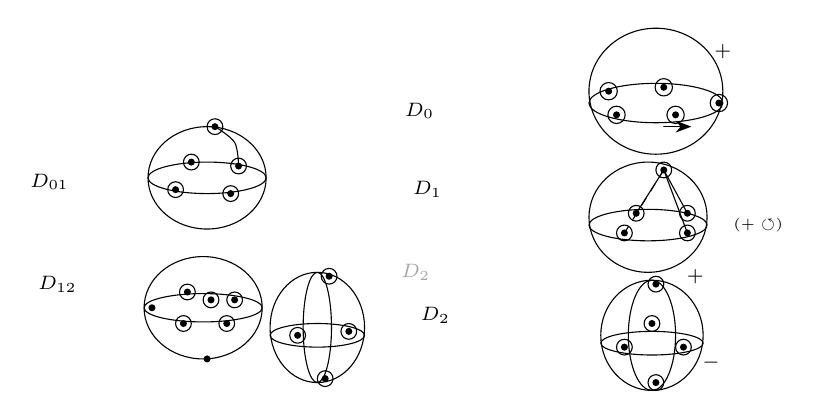
\begin{tikzpicture}[x=1mm,y=1mm,line cap=round,line join=round,font=\scriptsize]
\draw (26,-19.5) ellipse[x radius=7.5, y radius=6.5];
\draw (26,-19.5) ellipse[x radius=7.5, y radius=2];
\draw (24,-17.5) circle[radius=1];
\draw (30,-18) circle[radius=1];
\draw (22,-21) circle[radius=1];
\draw (29,-21.5) circle[radius=1];
\draw (27,-13) circle[radius=1];
\node[pt] at (24,-17.5) {};
\node[pt] at (30,-18) {};
\node[pt] at (22,-21) {};
\node[pt] at (29,-21.5) {};
\node[pt] at (27,-13) {};
\draw plot[smooth, tension=0.55] coordinates {(27,-13) (29.5,-15) (30,-18)};
\node[inner sep=1pt] at (6,-20) {\scriptsize $D_{01}$};
\draw (25.5,-36) ellipse[x radius=7.5, y radius=6.5];
\draw (25.5,-36) ellipse[x radius=7.5, y radius=1.8];
\draw (23.5,-34) circle[radius=1];
\draw (29.5,-35) circle[radius=1];
\draw (23,-38) circle[radius=1];
\draw (28.5,-38) circle[radius=1];
\draw (26.5,-35) circle[radius=1];
\node[pt] at (23.5,-34) {};
\node[pt] at (29.5,-35) {};
\node[pt] at (23,-38) {};
\node[pt] at (28.5,-38) {};
\node[pt] at (26.5,-35) {};
\node[pt] at (19,-36) {};
\node[pt] at (26,-42.5) {};
\draw (40,-38.5) ellipse[x radius=6, y radius=7];
\draw (40,-38.5) ellipse[x radius=1.8, y radius=7];
\draw (40,-39.5) ellipse[x radius=6, y radius=1.5];
\draw (37.5,-39.5) circle[radius=1];
\draw (44,-39) circle[radius=1];
\draw (41.5,-32) circle[radius=1];
\draw (41,-45) circle[radius=1];
\node[pt] at (37.5,-39.5) {};
\node[pt] at (44,-39) {};
\node[pt] at (41.5,-32) {};
\node[pt] at (41,-45) {};
\node[inner sep=1pt] at (7,-33) {\scriptsize $D_{12}$};
\draw (83,-8.5) ellipse[x radius=8.5, y radius=8];
\draw (83,-10) ellipse[x radius=8.5, y radius=2.5];
\draw (77,-8.5) circle[radius=1.1];
\draw (84,-8) circle[radius=1.1];
\draw (78,-11.5) circle[radius=1.1];
\draw (85.5,-11.5) circle[radius=1.1];
\draw (91,-10) circle[radius=1.1];
\node[pt] at (77,-8.5) {};
\node[pt] at (84,-8) {};
\node[pt] at (78,-11.5) {};
\node[pt] at (85.5,-11.5) {};
\node[pt] at (91,-10) {};
\draw[-{Stealth[length=2mm]}] (84,-13) -- (87.5,-13);
\node[inner sep=1pt] at (91.5,-3.5) {\scriptsize $+$};
\node[inner sep=1pt] at (53,-11) {\scriptsize $D_0$};
\draw (82,-24.5) ellipse[x radius=7.5, y radius=7];
\draw (82,-25.5) ellipse[x radius=7.5, y radius=2];
\draw plot[smooth, tension=0.55] coordinates {(84,-18.5) (80.5,-24)};
\draw plot[smooth, tension=0.55] coordinates {(84,-18.5) (87,-24)};
\draw[dashed] plot[smooth, tension=0.55] coordinates {(84,-18.5) (79,-26.5)};
\draw plot[smooth, tension=0.55] coordinates {(84,-18.5) (87,-26.5)};
\draw (84,-18.5) circle[radius=1];
\draw (80.5,-24) circle[radius=1];
\draw (87,-24) circle[radius=1];
\draw (79,-26.5) circle[radius=1];
\draw (87,-26.5) circle[radius=1];
\node[pt] at (84,-18.5) {};
\node[pt] at (80.5,-24) {};
\node[pt] at (87,-24) {};
\node[pt] at (79,-26.5) {};
\node[pt] at (87,-26.5) {};
\node[inner sep=1pt] at (54,-21) {\scriptsize $D_1$};
\node[inner sep=1pt] at (96,-25.5) {\tiny $(+\circlearrowleft)$};
\draw (82.5,-39.5) ellipse[x radius=6.5, y radius=7];
\draw (82.5,-39.5) ellipse[x radius=3, y radius=7];
\draw (82.5,-40.5) ellipse[x radius=6.5, y radius=1.5];
\draw (83,-33) circle[radius=1];
\draw (82.5,-38) circle[radius=1];
\draw (79,-41) circle[radius=1];
\draw (86.5,-41) circle[radius=1];
\draw (83,-45.5) circle[radius=1];
\node[pt] at (83,-33) {};
\node[pt] at (82.5,-38) {};
\node[pt] at (79,-41) {};
\node[pt] at (86.5,-41) {};
\node[pt] at (83,-45.5) {};
\node[inner sep=1pt,struck] at (52.5,-31.5) {\scriptsize $D_2$};
\node[inner sep=1pt] at (55,-37) {\scriptsize $D_2$};
\node[inner sep=1pt] at (88,-32) {\scriptsize $+$};
\node[inner sep=1pt] at (90,-43) {\scriptsize $-$};
\end{tikzpicture}
\end{document}
